% ASHG 2026 poster. Build: ASHG/build.sh  (diagrams from components/*.tex; logos in
% ASHG/poster/logos/, untracked; result figures from results/figures/poster/).
% Size: ASHG 2026 recommended poster 72 in wide x 36 in tall (board 96 x 48 in, landscape).
\documentclass{article}
\usepackage[paperwidth=72in, paperheight=36in, margin=0in]{geometry}
\usepackage[T1]{fontenc}
\usepackage{lmodern}                      % scalable math fonts (CM stops at 25pt)
% lmodern fixes the math-extension font (big delimiters) at 10pt; let it scale with the text
\DeclareFontFamily{OMX}{lmex}{}
\DeclareFontShape{OMX}{lmex}{m}{n}{<->lmex10}{}
\usepackage[default]{sourcesans}          % sans-serif body font (scalable)
\usepackage{amsmath, amssymb}
\usepackage{graphicx}
\usepackage{xcolor}
\usepackage{tcolorbox}
\tcbuselibrary{skins, fitting}
\tcbuselibrary{poster}
\usepackage{enumitem}
\usepackage{qrcode}
\usepackage{fontawesome5}
\usepackage{booktabs, array}
\usepackage{ragged2e}

\graphicspath{{../../results/figures/}{logos/}{components/}}
% Relationship-type colours shared by the pedigrees and the poster (Okabe-Ito, colour-blind safe).
\definecolor{cFull}{HTML}{0072B2}   % full siblings
\definecolor{cHalf}{HTML}{009E73}   % half-siblings
\definecolor{cStep}{HTML}{D55E00}   % step-siblings
\definecolor{cAdopt}{HTML}{56B4E9}  % adoptive siblings
\definecolor{cCous}{HTML}{CC79A7}   % 1st cousins
\definecolor{cCoc}{HTML}{E69F00}    % co-cousins
\definecolor{ink}{HTML}{1F2328}
% Variance-component colours, as in the stacked bar plots (fill; darker shade for text)
\definecolor{cAdd}{HTML}{4C8CB5}   \definecolor{cAddText}{HTML}{1F4E6E}   % additive (A)
\definecolor{cGxG}{HTML}{E3894B}   \definecolor{cGxGText}{HTML}{9A4A14}   % GxG
\definecolor{cFam}{HTML}{6FAF7A}   \definecolor{cFamText}{HTML}{2F6B3A}   % family environment
   % relative-type colours, shared with the pedigrees

% ---- colours (figure palette: ours = teal, Eftedal = salmon) ------------------------------
\definecolor{navy}{HTML}{1F3A5F}
\definecolor{teal}{HTML}{00A1B0}
\definecolor{salmon}{HTML}{E8685F}
\definecolor{paper}{HTML}{F6F7F9}
\definecolor{ink}{HTML}{1F2328}

% ---- type sizes (pt): body ~36pt is readable from ~2 m ------------------------------------
\newcommand{\bodysize}{\fontsize{34}{43}\selectfont}
\newcommand{\smallsize}{\fontsize{26}{32}\selectfont}
\newcommand{\boxtitlesize}{\fontsize{48}{56}\selectfont}
\newcommand{\titlesize}{\fontsize{100}{116}\selectfont}
\newcommand{\authorsize}{\fontsize{50}{60}\selectfont}

\setlist[itemize]{leftmargin=1.1em, itemsep=0.35em, topsep=0.3em, label={\color{teal}\textbullet}}
\newcommand{\takeaway}[1]{\par\smallskip{\color{navy}\bfseries #1}\par}
\newcommand{\eftedal}{{\color{salmon}\bfseries Eftedal}}
\newcommand{\ours}{{\color{teal}\bfseries ours}}

\pagestyle{empty}
\frenchspacing
\color{ink}

\begin{document}
\begin{tcbposter}[
  coverage = {spread, interior style={fill=paper}},
  poster = {columns=20, rows=36, spacing=1.2cm},
  boxes = {enhanced, arc=6mm, boxrule=0pt, colback=white, colframe=navy,
           fonttitle=\boxtitlesize\bfseries, coltitle=white,
           left=12mm, right=12mm, top=10mm, bottom=10mm, toptitle=5mm, bottomtitle=5mm,
           fontupper=\bodysize, before upper={\parskip=0.5em}}
]

% ============================== HEADER ==============================
\posterbox[blankest, interior engine=empty, colback=navy, colupper=white,
           underlay={\fill[navy] (frame.south west) rectangle (frame.north east);},
           halign=center, valign=center]
  {name=header, column=1, span=20, row=1, rowspan=6}{%
  \hspace*{1.3in}%
  \begin{minipage}[c]{0.13\linewidth}\raggedright
    \includegraphics[height=1.9in]{hms_dark}\\[0.4in]
    \includegraphics[height=1.55in]{dfci_dark}
  \end{minipage}\hfill
  \begin{minipage}[c]{0.58\linewidth}\centering
    {\titlesize\bfseries Relatives\textquoteright{} similarity in test score performance is explained by\\[0.15em]
     a wide range of genetic and environmental parameters\par}
    \vspace{0.5em}
    {\authorsize Nuno R.\,G. Carvalho\textsuperscript{1,2} \quad and \quad Alexander ``Sasha'' Gusev\textsuperscript{1,2}\par}
    \vspace{0.2em}
    {\fontsize{36}{44}\selectfont \textsuperscript{1}Harvard Medical School \quad \textsuperscript{2}Dana-Farber Cancer Institute\par}
  \end{minipage}\hfill
  \begin{minipage}[c]{0.235\linewidth}\raggedright
    \begin{minipage}[c]{0.66\linewidth}\RaggedRight\fontsize{25}{30}\selectfont
      \textbf{Based on:} Eftedal NH, Eilertsen EM, Sunde HF, Kleppest\o{} TH, Ystrom E, Czajkowski NO (2025).
      Beyond additive genetic effects: Explaining family resemblance in school performance across
      millions of pairs of Norwegian relatives. \textit{PNAS} 122(25):e2419627122.\par\medskip
      \faTwitter\ @nunorgcarvalho\par
      \faEnvelope\ nuno\_ramosgrangeiacarvalho@\allowbreak g.harvard.edu\par
    \end{minipage}\hspace{0.35in}%
    \begin{minipage}[c]{0.28\linewidth}\centering
      % TODO: point to the public repository / ePoster once available
      \colorbox{white}{\color{black}\qrcode[height=2.4in]{https://github.com/nunorgcarvalho/eftedal_reanalysis}}\\[0.2em]
      {\fontsize{25}{30}\selectfont Supplementary Material}
    \end{minipage}
  \end{minipage}\hspace*{0.3in}%
}

% ============================== helpers ==============================
% swatch in a relative-type colour (matches the pedigree connectors)
\newcommand{\relswatch}[1]{\textcolor{#1}{\rule[0.18em]{1.6em}{0.32em}}}
\newcommand{\relname}[2]{\relswatch{#1}\hspace{0.5em}{\color{#1}\bfseries #2}}
\newcommand{\tablesize}{\fontsize{30}{38}\selectfont}
\newcommand{\subhead}[1]{{\color{navy}\bfseries\fontsize{40}{48}\selectfont #1\par}\smallskip}
\newcommand{\refcite}[1]{{\color{navy}[#1]}}

% ============================== ROW 1: background (vertical banner) ==============================
\newcommand{\bgsize}{\fontsize{31}{37}\selectfont}
\posterbox[notitle, left=3.6cm, right=10mm, top=6mm, bottom=6mm, valign=center, fontupper=\bgsize,
           before upper={\parskip=0.3em},
           overlay={\begin{tcbclipframe}\fill[navy] (frame.south west) rectangle ([xshift=2.5cm]frame.north west);\end{tcbclipframe}
                    \node[rotate=90, text=white, font=\boxtitlesize\bfseries] at ([xshift=1.25cm]frame.west) {Background};}]
  {name=bg, column=1, span=20, row=7, rowspan=6}{%
\begin{minipage}[c]{0.17\linewidth}\raggedright
\setlist[itemize]{leftmargin=0.9em, itemsep=0.25em, topsep=0.1em}
Relatives have similar test scores due to shared genetics and shared environments\par\vspace{0.6em}
\refcite{Eftedal et al.\ 2025, \textit{PNAS}} fit the \textbf{Additive model} to school test scores of
        $\sim$1M Norwegian children
\begin{itemize}
  \item identified the relative type of each pair of relatives
  \item fit the observed correlations by relative type as a function of the Additive model's parameters
\end{itemize}
\end{minipage}\hfill
\begin{minipage}[c]{0.125\linewidth}\centering\includegraphics[width=\linewidth]{pedigree_sibs}\end{minipage}\hfill
\begin{minipage}[c]{0.16\linewidth}\centering\includegraphics[width=\linewidth]{pedigree_cousins}\end{minipage}\hfill
\begin{minipage}[c]{0.155\linewidth}\centering
{\fontsize{30}{35}\selectfont\renewcommand{\arraystretch}{1.42}\setlength{\tabcolsep}{0.4em}%
\begin{tabular}[t]{@{}l c c >{$}l<{$}@{}}
\toprule
\textbf{relatives} & $\boldsymbol{n}$ & $\boldsymbol{f}$ & \text{\textbf{correlation implied}} \\[-0.55em]
                   &                  &                  & \text{\textbf{by Additive model}} \\
\midrule
\relname{cFull}{full siblings}      & 1   & 0   & V_A\,(1+m)/2 \\
\relname{cHalf}{half-siblings}      & 2   & 0.5 & V_A\,(1+2m+rm)/4 \\
\relname{cStep}{step-siblings}      & 1+1 & 1   & V_A\,m\,\big((1+r)/2\big)^{2} \\
\relname{cAdopt}{adoptive siblings} & --  & 0   & 0 \\
\relname{cCous}{1st cousins}        & 3   & 1   & V_A\,\big((1+m)/2\big)^{3} \\
\relname{cCoc}{co-cousins}          & 2+2 & 2   & V_A\,m\,\big((1+m)/2\big)^{4} \\
\bottomrule
\end{tabular}\par}
\end{minipage}\hfill
\begin{minipage}[c]{0.2\linewidth}
\subhead{Two types of fits}
{\fontsize{30}{35}\selectfont\renewcommand{\arraystretch}{1.2}\setlength{\tabcolsep}{0.3em}%
\begin{tabular}{@{}>{\bfseries\raggedright\arraybackslash}p{0.2\linewidth} >{\raggedright\arraybackslash}p{0.37\linewidth} >{\raggedright\arraybackslash}p{0.37\linewidth}@{}}
\toprule
 & \textbf{Marginal Pair} & \textbf{Marginal Type} \\
\midrule
unit & each \textbf{pair} of relatives & each \textbf{relative type} \\
weights & $1/SE^2$ & uniform across types \\
95\% CI & parametric bootstrap & leave-one-type-out jackknife\\
use & within-model comparisons & \textbf{across-model comparisons} \\
\bottomrule
\end{tabular}\par}
\end{minipage}\hfill
\begin{minipage}[c]{0.175\linewidth}\raggedright
\subhead{Problems in Eftedal et al.'s estimator}
\setlist[itemize]{leftmargin=0.9em, itemsep=0.2em, topsep=0.1em}
\begin{itemize}
  \item Only optimized for Marginal Pair, not Marginal Type
  \item Log-transformed correlations: over-weights distant relatives
  \item Incorrect inverse-variance weights: over-weight distant relatives
  \item Incorrect expected correlation for step-siblings
  \item Phenotypic ($r$) and genetic ($m$) correlations between mates estimated independently,
        although the model implies $m = V_A\,r$
  % optional additions (uncomment if wanted):
  % \item Relatives through twins of unknown zygosity left out of the fit
  % \item CIs from resampling relative categories in proportion to $1/SE^2$
\end{itemize}
\end{minipage}%
}

% ============================== ROWS 2-4 ==============================
% columns 18-20: key above takeaways
\posterbox[adjusted title=Takeaways, fontupper=\fontsize{31}{38}\selectfont]{name=take, column=18, span=3, above=bottom}{
\begin{itemize}
  \item Revising Eftedal et al.'s estimator for the Additive model yields \textbf{high $V_A$}
        estimates that explain different relative types better
  \item Additive, GxG and shared-environment components are \textbf{collinear}: weak evidence for
        significant components beyond the Additive model
  \item No single model fully explains correlations across all relative types
\end{itemize}
}

\newcommand{\keyswatch}[1]{\textcolor{#1}{\rule[-0.05em]{0.75em}{0.75em}}}
\newcommand{\keysym}[3]{\keyswatch{#1}\hspace{0.4em}{\color{#2}$#3$}}
\posterbox[adjusted title=Key]{name=key, column=18, span=3, between=bg and take}{
\centering{\fontsize{36}{42}\selectfont\renewcommand{\arraystretch}{1.7}%
\begin{tabular}{@{}l >{\raggedright\arraybackslash}p{0.66\linewidth}@{}}
\toprule
\textbf{symbol} & \textbf{meaning} \\
\midrule
\multicolumn{2}{@{}l}{\textit{\color{cAddText}Additive model}} \\
\keysym{cAdd}{cAddText}{n}   & genetic degree \\
\keysym{cAdd}{cAddText}{V_A} & additive genetic variance \\
\keysym{cAdd}{cAddText}{V_A^0} & additive variance under random mating, $V_A(1-m)$ \\
\keysym{cAdd}{cAddText}{m}   & mates' genetic correlation \\
\keysym{cAdd}{cAddText}{r}   & mates' phenotypic correlation \\
\midrule
\multicolumn{2}{@{}l}{\textit{\color{cGxGText}Gene--gene interactions}} \\
\keysym{cGxG}{cGxGText}{V_{\mathrm{GxG}}} & GxG variance \\
\midrule
\multicolumn{2}{@{}l}{\textit{\color{cFamText}Shared environment}} \\
\keysym{cFam}{cFamText}{V_C} & shared-environment variance \\
\keysym{cFam}{cFamText}{f}   & family degree \\
\keysym{cFam}{cFamText}{c} & decay per family degree \\
\bottomrule
\end{tabular}\par}
}

% columns 1-7: revising Eftedal et al. (figure)
\posterbox[adjusted title=Revising Eftedal et al.'s results]{name=rev, column=1, span=7, between=bg and bottom}{
\subhead{Additive model: Eftedal et al.\ vs.\ revised}
The Revised estimator fixes errors in Eftedal et al.'s estimator and is optimized for the Marginal Type.\par\smallskip
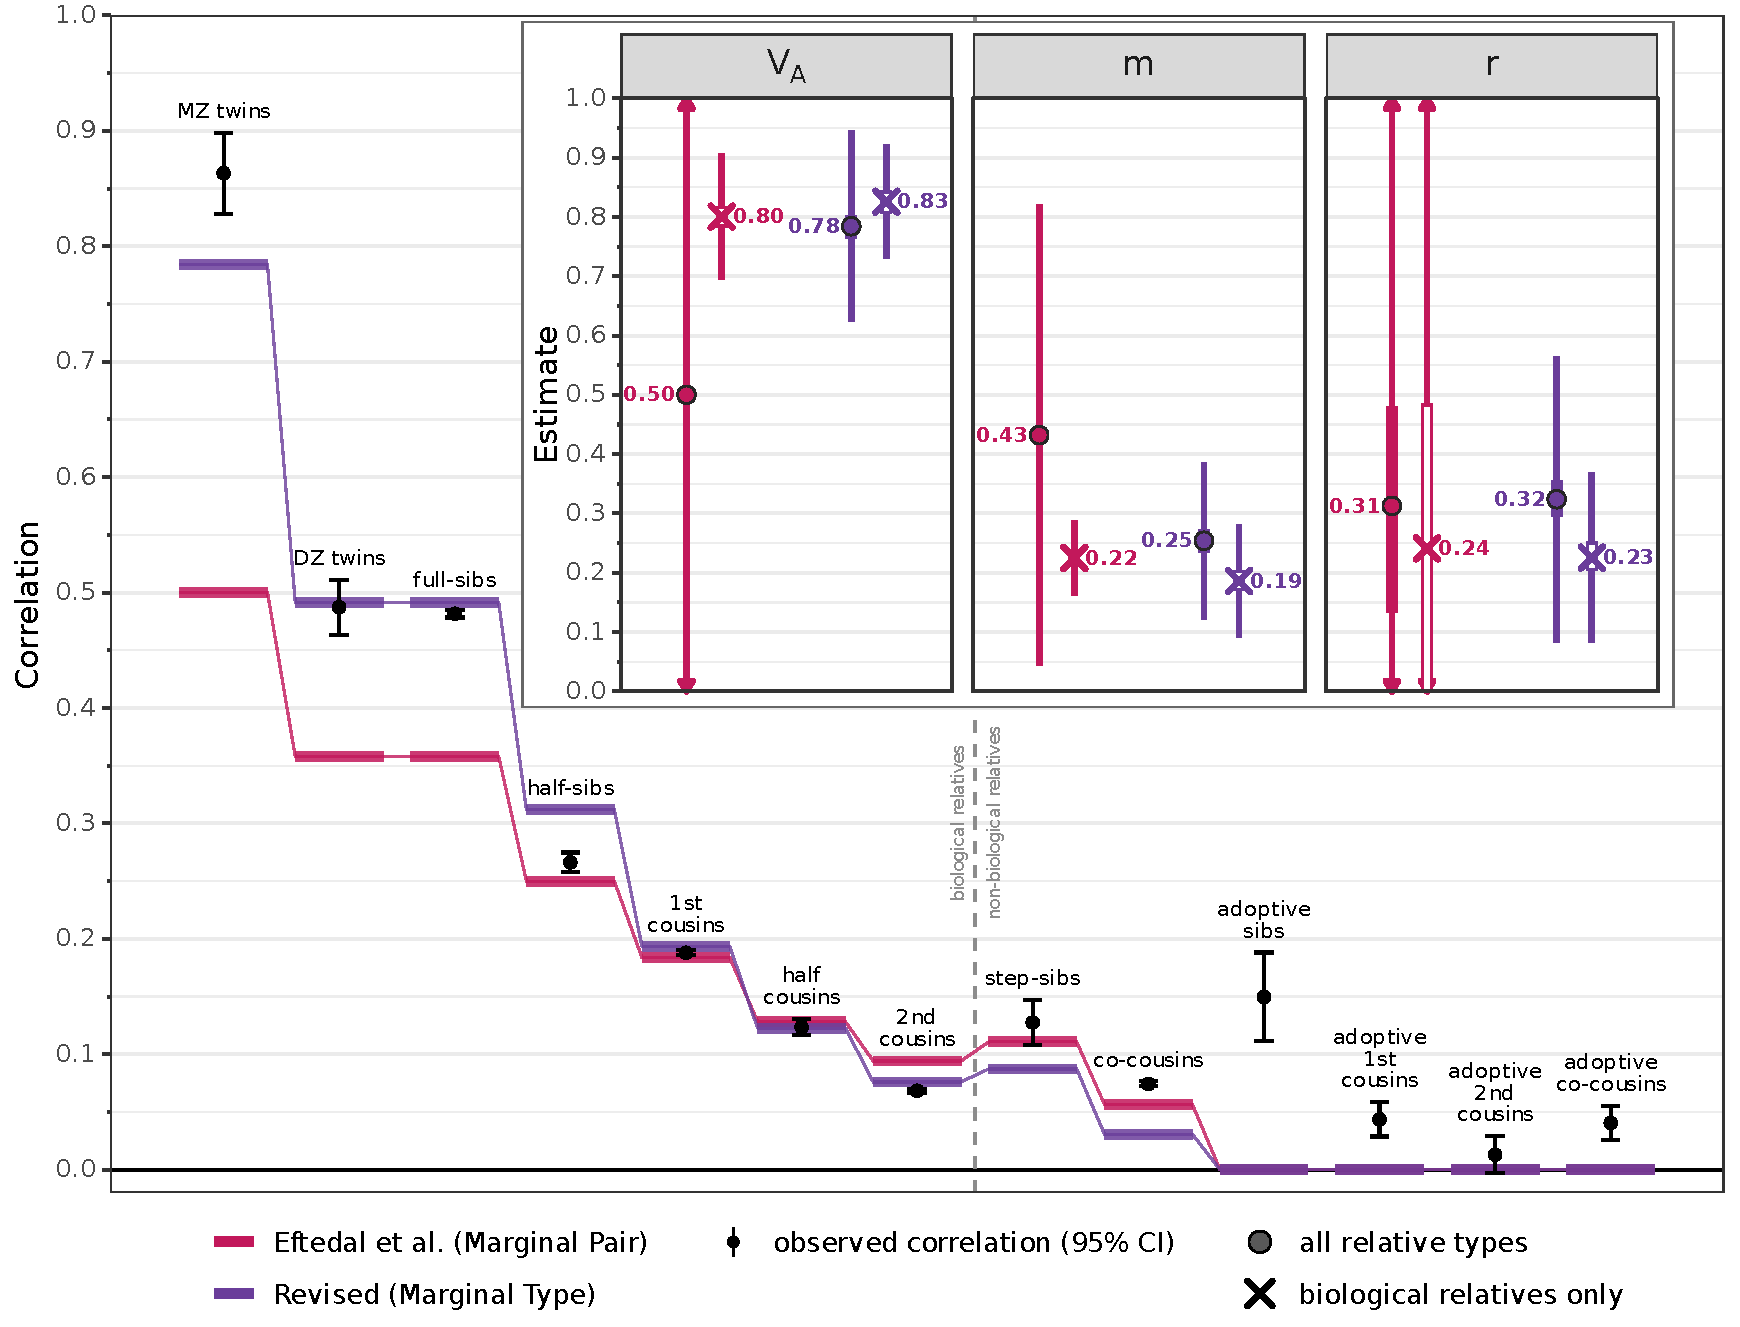
\includegraphics[width=\linewidth]{poster/p4_fit_and_params}\par
{\smallsize Colored bars denote each model's predicted correlation for each relative type.
Actual observed correlations shown in black.
Eftedal et al.'s estimator optimizes for the Marginal Pair, while the Revised estimator optimizes for the Marginal Type.

Inset: parameter estimates compared between training cohorts, as done in Eftedal et al.: biological relatives only vs.\ all relative types.
Both types of CIs are shown.\par}
}

% columns 8-17: models with GxG and shared environment
\posterbox[adjusted title=Models with GxG and shared environment]{name=gxg, column=8, span=10, between=bg and bottom}{
\begin{minipage}[t]{0.33\linewidth}
\subhead{\color{cGxGText}Gene--gene interactions (GxG)}
Pairwise genetic interactions, not affected by assortative mating (AM).
{\fontsize{44}{52}\selectfont\[ \rho_k = \dots + V_{\mathrm{GxG}}\left(\frac{1}{4}\right)^{n_k} \]}

\vspace{1.0em}
\subhead{\color{cFamText}Shared environment (C)}
Environment shared across the extended family, decaying at a rate of $c$ with respect to family degree $f$:
{\fontsize{44}{52}\selectfont\[ \rho_k = \dots + V_C\, c^{\,f_k} \]}%
\noindent Can be decomposed into within-sibling ($V_C(1-c)$) vs.\ beyond-sibling ($V_C\,c$) shared environment.

\vspace{1.0em}
\subhead{Variance components}
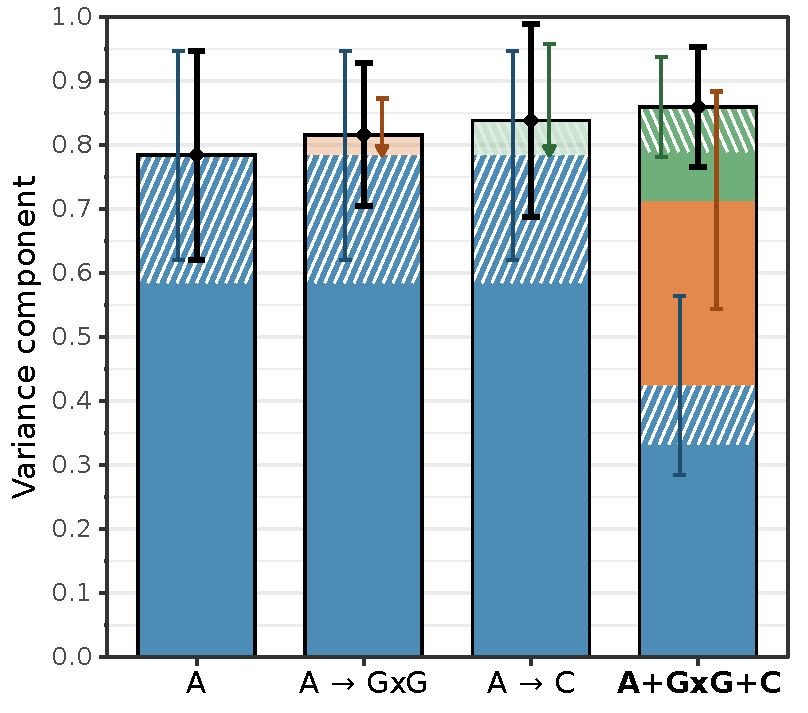
\includegraphics[width=\linewidth]{poster/p6_components_four_models}\par
{\smallsize A $\rightarrow$ B indicates two-step estimation, fixing A first.
Marginal Type point estimates and 95\% CIs.
Color is faded if component variance is not significantly greater than 0.
Black indicates sum of variance components.
A+GxG+C is bolded and used as the example in the adjacent figure.\par}
\end{minipage}\hfill
\begin{minipage}[t]{0.645\linewidth}
\subhead{Example: A+GxG+C}
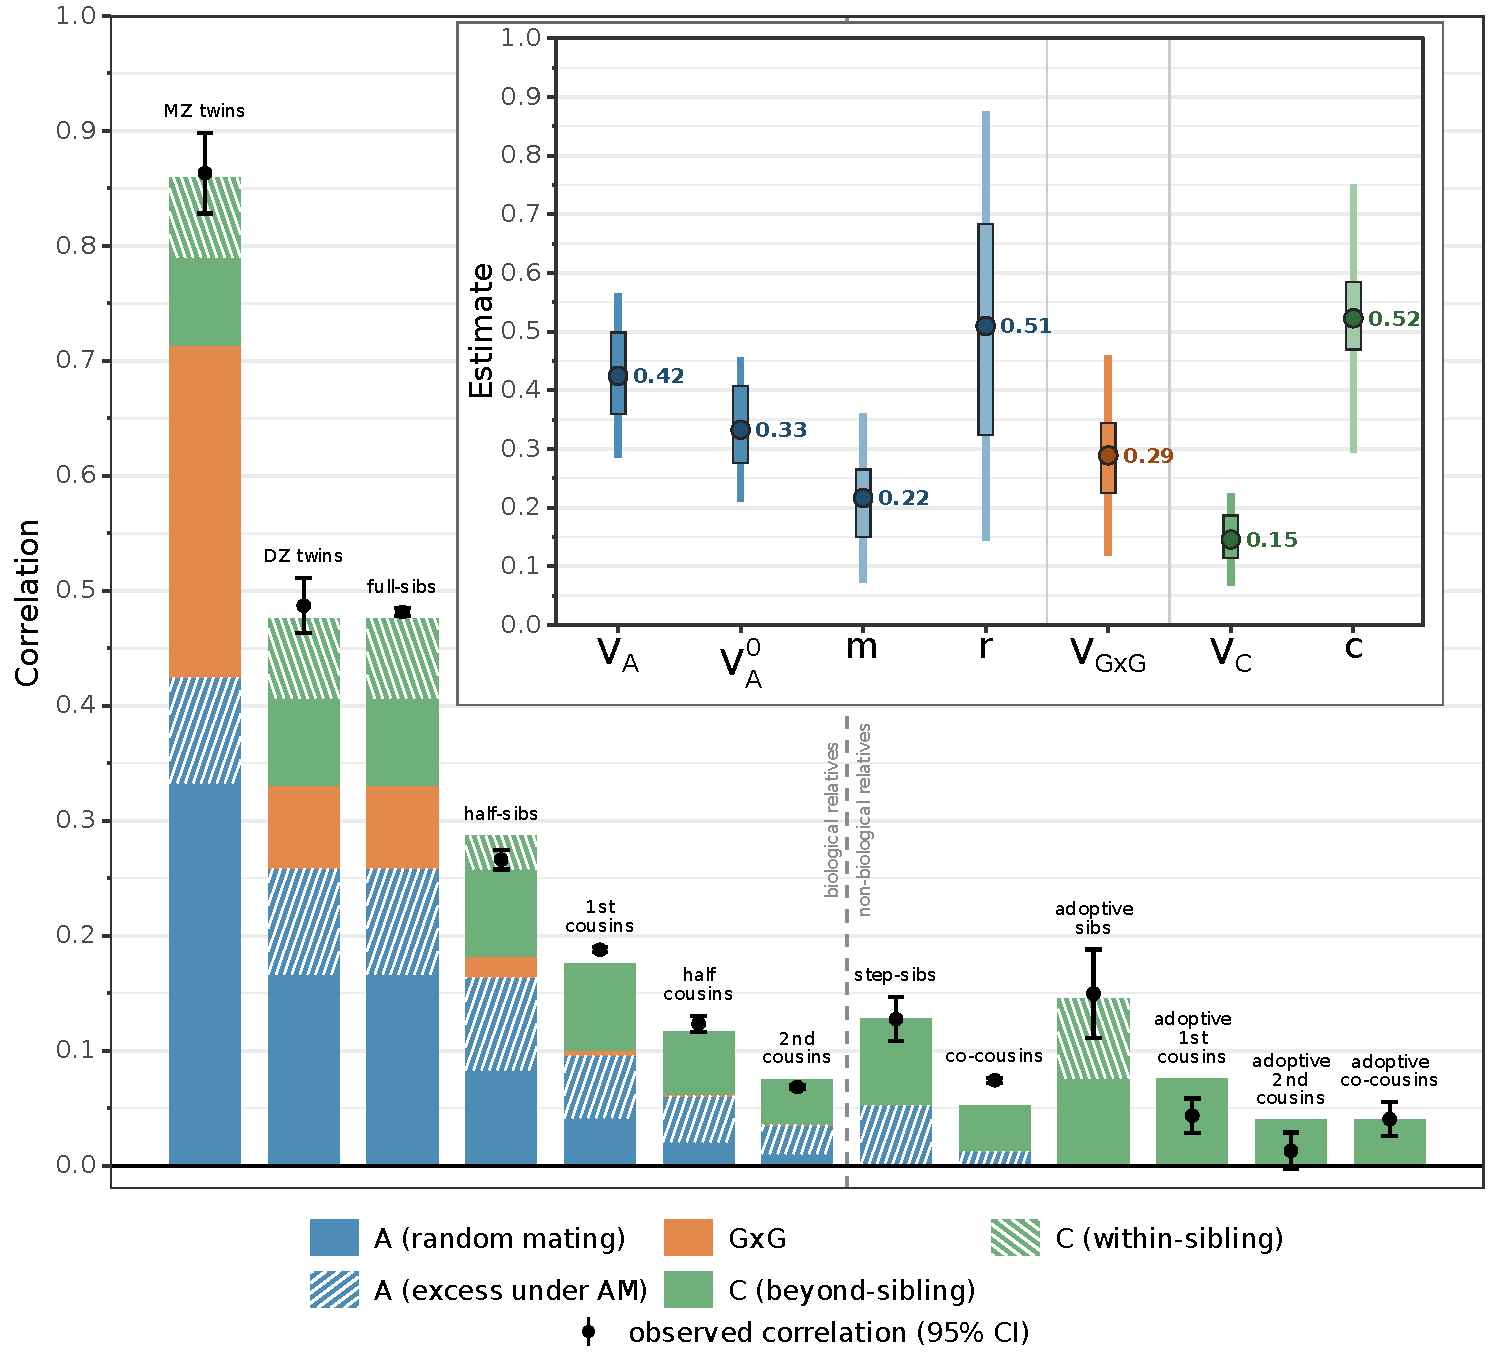
\includegraphics[width=\linewidth]{poster/p5_components_and_params}\par
{\smallsize Predicted correlation of each relative type, decomposed by component.
Marginal Type fit.
 Inset: parameter estimates; both types of CIs are shown.\par}
\end{minipage}
}

\end{tcbposter}
\end{document}
